\documentclass[final]{article}

\usepackage{aps360}               % course style: ../aps360.sty, found via latexmkrc
\usepackage[utf8]{inputenc}
\usepackage[T1]{fontenc}
\usepackage{hyperref}
\usepackage{url}
\usepackage{booktabs}
\usepackage{amsmath}
\usepackage{amsfonts}
\usepackage{nicefrac}
\usepackage{microtype}
\usepackage{xcolor}
\usepackage{graphicx}
\usepackage{caption}
\usepackage{etoolbox}
\usepackage{tikz}
\usetikzlibrary{arrows.meta, positioning, calc}

\captionsetup{font=small, skip=2pt}               % space between a figure/table and its caption
\setlength{\intextsep}{3pt plus 1pt minus 1pt}     % space between text and in-text floats
\setlength{\textfloatsep}{4pt plus 1pt minus 1pt}  % space between text and top/bottom floats
\setlength{\floatsep}{3pt plus 1pt minus 1pt}      % space between two floats
\renewcommand{\bottomfraction}{0.5}  % let a large figure sit at the bottom of a page
\setcounter{totalnumber}{5}           % default allows only 3 floats per page
\setcounter{bottomnumber}{2}
\AtBeginDocument{\setcitestyle{numbers, square}}   % after aps360.sty's own natbib setup
\graphicspath{{figures/}}

% aps360.sty expects a conference-track option that the course template never sets
\makeatletter
\providecommand{\@trackname}{APS360 Project Progress Report}
% the style's 2 extra lines meant for page 1 land on page 2 here and hit the page number
\patchcmd{\@notice}{\enlargethispage{2\baselineskip}}{}{}{\PackageError{main}{notice patch failed}{}}
\makeatother

\title{Floor Segmentation for AR-Style Indoor and Outdoor Navigation}

\author{%
  Lancelot Shih \\
  1008759817, \texttt{lancelot.shih@mail.utoronto.ca} \\
  Code: \texttt{https://github.com/LancelotShih/NavAR}
}

\begin{document}

\maketitle
\vspace{-0.45in}

% =====================================================================
\section*{Brief Project Description}

In our ever increasingly more detailed world, we rely more and more on tools like Google Maps to 
navigate the world. Fundamentally, that means we are tied to our phone and there is not 
really a way around that. However, as Augmented Reality (AR) systems become increasingly more
mainstream, the goal of this project is to capture a pathway over a live camera view as an 
intuitive way to navigate the world. Such an overlay first needs to know \emph{where the floor is}. 
Thus, this project builds a network that takes a single RGB photo, indoors or outdoors, 
and outputs a per-pixel floor mask (Figure~\ref{fig:overview}).

Deep learning suits the task because ``floor'' has no fixed appearance as carpet, tile, wood and
concrete differ completely, and a grey wall can look almost identical to a grey floor. Telling them apart
needs scene context, such as where the walls meet the ground, and what is standing on the floor, which 
a convolutional encoder--decoder learns from labelled examples while a simple colour rule cannot.

\begin{figure}[h]
  \centering
  \begin{tikzpicture}[font=\small, >={Stealth[length=2mm]},
      box/.style={draw, rounded corners=2pt, fill=blue!6, align=center, inner sep=4pt}]
    \node (in)  {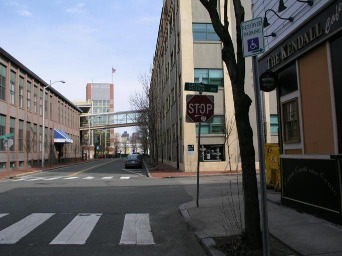
\includegraphics[width=2.9cm]{overview_input.jpg}};
    \node[box, right=0.55cm of in] (net) {U-Net\\[-1pt]{\scriptsize ResNet-34 encoder}\\[-1pt]{\scriptsize (ImageNet-pretrained)}\\[-1pt]{\scriptsize + skip-connected decoder}};
    \node[right=0.55cm of net] (out) {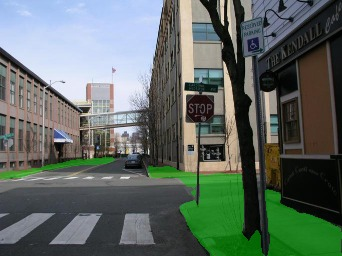
\includegraphics[width=2.9cm]{overview_output.jpg}};
    \draw[->, thick] (in) -- (net);
    \draw[->, thick] (net) -- (out);
    \node[below=0pt of in,  font=\scriptsize] {input: RGB photo, any size};
    \node[below=0pt of out, font=\scriptsize] {output: floor probability per pixel $>0.5$ (green)};
  \end{tikzpicture}
  \caption{Input and output on a validation street scene: sidewalks are floor; road and crosswalk are not.}
  \label{fig:overview}
\end{figure}

% =====================================================================
\section*{Notable Contribution}

\subsection*{Data Processing}


\textbf{Source.} I used the ADE20K scene-parsing release~\citep{zhou2017ade20k} that included 20,210 training
and 2,000 validation photos (indoor and outdoor) with per-pixel labels for 150 classes. Its test
labels are not public, so the official validation set is my test set, and a random
10\% of the training images (shuffled with a fixed random seed of 0) turns into my validation set for 
model selection. All reported scores currently use my validation set.

\textbf{Cleaning.} Each 150-class mask is merged into three values

\emph{floor} = floor, rug, sidewalk, path

\emph{ignore} = unlabelled and ambiguous ground (stairs, stairway, step, escalator, grass, earth, field, sand)

\emph{not floor} = every other class, including road, because the target user is a pedestrian.

Ignored pixels are excluded from loss and metrics. Images without floor are kept so the
model learns to predict nothing. Masks are cached as PNGs and splits are fixed by ID lists
(Table~\ref{tab:data}, Figure~\ref{fig:samples}).

\textbf{Formatting.} Images are resized to a shorter side of 256px (masks with nearest-neighbour)
and normalised with ImageNet statistics. Training adds a random $256{\times}256$ crop, horizontal
flip and mild colour jitter (brightness/contrast/saturation $\pm 0.2$, hue $\pm 0.02$). I did no
vertical flip since floor is almost always at the bottom of the frame. Evaluation uses the whole
image, padded to a multiple of 32 with ignored pixels.

\begin{table}[h]
  \centering\small
  \caption{Cleaned data. ``No floor'': images with no floor pixel at all. Pixel shares are of all pixels.}
  \label{tab:data}
  \begin{tabular}{lrrrrr}
\toprule
Split & Images & No floor & Floor px & Not-floor px & Ignored px \\
\midrule
Train & 18,189 & 36.3\% & 8.4\% & 78.7\% & 13.0\% \\
Validation & 2,021 & 35.5\% & 8.2\% & 79.1\% & 12.6\% \\
Test (held out) & 2,000 & 35.4\% & 8.7\% & 78.6\% & 12.7\% \\
\bottomrule
\end{tabular}

\end{table}

\begin{figure}[h]
  \centering
  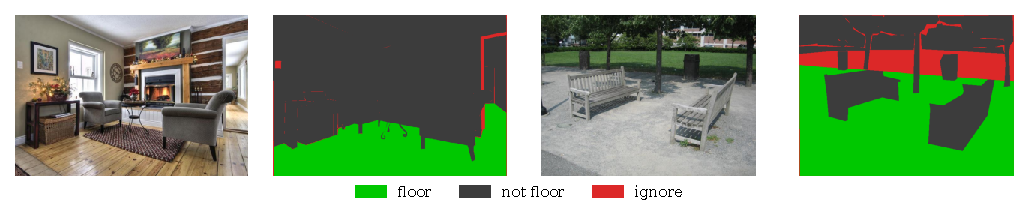
\includegraphics[width=\linewidth]{data_samples.pdf}
  \caption{Cleaned training samples (photo, merged mask): the rug joins the floor; park grass is ignored.}
  \label{fig:samples}
\end{figure}

\textbf{Plan for unseen data.} For the final report I will evaluate the chosen model once on
the 2,000 held-out ADE20K test images and record phone video on campus, indoors and outdoors,
and hand-label about 100 frames under the same rules in various downtown Toronto settings.

\textbf{Challenges.} Since the floor is only 8\% of pixels and 36\% of images contain none, per-image
metrics are often undefined. Thus, IoU, precision, and recall are calculated by pooling pixel counts 
over the whole split.

% =====================================================================
\subsection*{Baseline Model}


The baseline is a hand-coded colour model with no learning (Figure~\ref{fig:baseline}). It assumes
the pixels at the bottom 20\% of rows and middle 30\% of columns are always floor, computes that
patch's mean colour $\mu$ in Lab space, and labels a pixel with colour $x$ as floor if its mean
squared error $\mathrm{MSE}(x) = \frac{1}{3}\sum_{c \in \{L,a,b\}} (x_c-\mu_c)^2$ is below a
threshold $\tau$. Its one parameter, $\tau$, was tuned on the validation set ($\tau = 200$).

\begin{figure}[h]
  \centering
  \begin{minipage}[c]{0.5\linewidth}
    \centering
    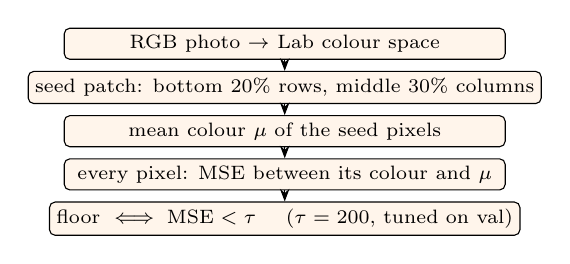
\begin{tikzpicture}[font=\scriptsize, >={Stealth[length=1.6mm]}, node distance=0.14cm,
        stage/.style={draw, rounded corners=2pt, fill=orange!8, align=center, minimum width=5.6cm, inner sep=2.5pt}]
      \node[stage] (a) {RGB photo $\rightarrow$ Lab colour space};
      \node[stage, below=of a] (b) {seed patch: bottom 20\% rows, middle 30\% columns};
      \node[stage, below=of b] (c) {mean colour $\mu$ of the seed pixels};
      \node[stage, below=of c] (d) {every pixel: MSE between its colour and $\mu$};
      \node[stage, below=of d] (e) {floor $\iff \mathrm{MSE} < \tau$ \quad ($\tau = 200$, tuned on val)};
      \foreach \x/\y in {a/b, b/c, c/d, d/e} \draw[->] (\x) -- (\y);
    \end{tikzpicture}
  \end{minipage}%
  \begin{minipage}[c]{0.48\linewidth}
    \centering
    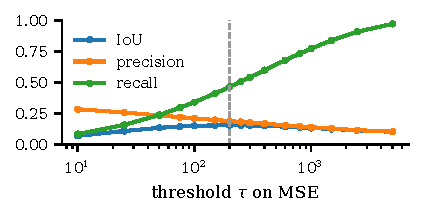
\includegraphics[width=\linewidth]{threshold.pdf}
  \end{minipage}
  \caption{Colour baseline: pipeline (left) and validation IoU, precision and recall against the
  threshold $\tau$ (right). Loosening $\tau$ raises recall but lowers precision; IoU peaks at $\tau = 200$.}
  \label{fig:baseline}
\end{figure}

It reaches a validation Intersection over Union (IoU) of only 0.15 (Table~\ref{tab:results}) with its largest 
sources of false alarms being walls (17\%), buildings (14\%) and roads (13\%). Note that the patch is mostly 
floor in only 28\% of images, and the model cannot tell when floor is absent. Tuning $\tau$ could not fix this,
as higher recall always costs precision.

% =====================================================================
\subsection*{Primary Model}

\textbf{Architecture.} A U-Net~\citep{ronneberger2015unet} whose encoder is a
ResNet-34~\citep{he2016resnet} pretrained on ImageNet~\citep{deng2009imagenet}, built with
\texttt{segmentation\_models\_pytorch}~\citep{iakubovskii2019smp} (Figure~\ref{fig:unet}). Each decoder block 
upsamples $2\times$ and applies two $3\times3$ conv--BatchNorm--ReLU layers, with the first four blocks 
concatenating the same resolution encoder features (skip connections) first. A final $3{\times}3$ convolution
gives one logit per pixel, and floor is predicted where its sigmoid exceeds 0.5. The network has 47 convolutional
layers and 24.4\,M parameters (21.3\,M in the encoder).

\begin{figure}[h]
  \centering
  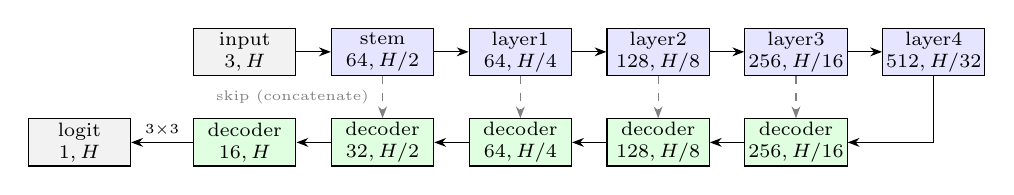
\begin{tikzpicture}[font=\scriptsize, >={Stealth[length=1.5mm]},
      blk/.style={draw, minimum width=1.3cm, minimum height=0.6cm, align=center, inner sep=1pt},
      enc/.style={blk, fill=blue!10}, dec/.style={blk, fill=green!12}, io/.style={blk, fill=gray!10}]
    \def\dx{1.75} \def\dy{1.15}
    % top row: encoder (resolution halves left to right)
    \node[io] (in) at (0, 0) {input\\$3, H$};
    \foreach \l/\t/\c/\r in {1/stem/64/H{/}2, 2/layer1/64/H{/}4, 3/layer2/128/H{/}8, 4/layer3/256/H{/}16, 5/layer4/512/H{/}32}
      \node[enc] (e\l) at ({\l*\dx}, 0) {\t\\$\c, \r$};
    % bottom row: decoder (resolution doubles right to left), each block under the encoder stage it matches
    \foreach \l/\c/\r in {4/256/H{/}16, 3/128/H{/}8, 2/64/H{/}4, 1/32/H{/}2, 0/16/H}
      \node[dec] (d\l) at ({\l*\dx}, -\dy) {decoder\\$\c, \r$};
    \node[io] (out) at ({-\dx-0.35}, -\dy) {logit\\$1, H$};
    \draw[->] (in) -- (e1);
    \foreach \a/\b in {1/2, 2/3, 3/4, 4/5} \draw[->] (e\a) -- (e\b);
    \draw[->] (e5.south) |- (d4.east);
    \foreach \a/\b in {4/3, 3/2, 2/1, 1/0} \draw[->] (d\a) -- (d\b);
    \draw[->] (d0) -- node[above=-1pt, font=\tiny] {$3{\times}3$} (out);
    \foreach \l in {1, 2, 3, 4} \draw[->, dashed, gray] (e\l) -- (d\l);
    \node[gray, font=\tiny, anchor=east] at ({1*\dx-0.05}, {-0.5*\dy}) {skip (concatenate)};
  \end{tikzpicture}
  \caption{U-Net with a ResNet-34 encoder (blue) and five upsampling decoder blocks (green); each box
  shows channels and resolution for an $H{\times}W$ input. Dashed arrows: skip connections.}
  \label{fig:unet}
\end{figure}

\textbf{Training.} Loss = binary cross-entropy + soft Dice~\citep{milletari2016vnet}, both averaged
over non-ignored pixels only (Dice is pooled over the batch, so floor-free images are handled).
AdamW~\citep{loshchilov2019adamw} (weight decay $10^{-4}$), batch 16, 30 epochs, learning rate
decayed to zero with a per-step cosine schedule~\citep{loshchilov2017sgdr}, mixed precision
(fp16)~\citep{micikevicius2018mixed}. The checkpoint with the best validation IoU is kept. One run
takes 48 minutes on a single RTX~3070 (8\,GB). A learning rate and batch size sweep
(Figure~\ref{fig:curves}b) chose $10^{-4}$ as $10^{-3}$ was clearly too high for fine-tuning the
pretrained encoder, and batch size made little difference.

\begin{figure}[h]
  \centering
  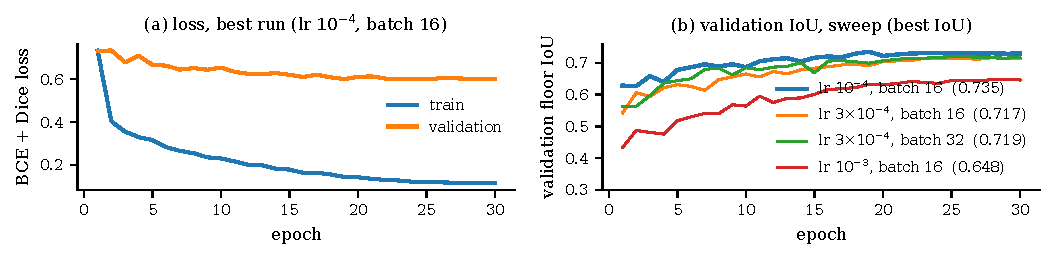
\includegraphics[width=\linewidth]{curves.pdf}
  \caption{(a) Validation loss flattens after epoch $\sim$20 while training loss keeps falling, but
  validation IoU dips only slightly after its peak (0.735 to 0.729), so the best checkpoint is not overfit. 
  (b) Validation IoU of each sweep run.}
  \label{fig:curves}
\end{figure}

\textbf{Results.} The U-Net reaches a validation IoU of 0.735, 4.8 times the baseline, with
precision 0.88 (Table~\ref{tab:results}). It recovers 85--90\% of indoor floor and rugs but only
52--67\% of sidewalks and paths. Roads are its largest source of false alarms (25\% of them), yet it
labels only 7\% of road pixels as floor. In Figure~\ref{fig:qualitative} the baseline spills onto
similarly coloured walls, beds and windows, while the U-Net follows floor boundaries indoors and
struggles mainly outdoors.

\begin{table}[h]
  \centering\small
  \setlength{\tabcolsep}{4.5pt}
  \caption{Validation results (2,021 images). Last column: share of the 717 floor-free images marked ${>}1\%$ floor.}
  \label{tab:results}
  \begin{tabular}{lrrrrrrrr}
\toprule
& & & & \multicolumn{4}{c}{Recall by surface (\%)} & No-floor imgs \\ \cmidrule(lr){5-8}
Method & IoU & Prec. & Rec. & floor & rug & sidewalk & path & w/ false floor \\
\midrule
Colour baseline & 0.155 & 0.188 & 0.465 & 45.4 & 46.3 & 51.0 & 49.0 & 99.9\% \\
\textbf{U-Net (ours)} & \textbf{0.735} & \textbf{0.879} & \textbf{0.818} & \textbf{85.4} & \textbf{90.1} & \textbf{67.1} & \textbf{52.2} & \textbf{22.6\%} \\
\bottomrule
\end{tabular}

\end{table}

\begin{figure}[!htb]
  \centering
  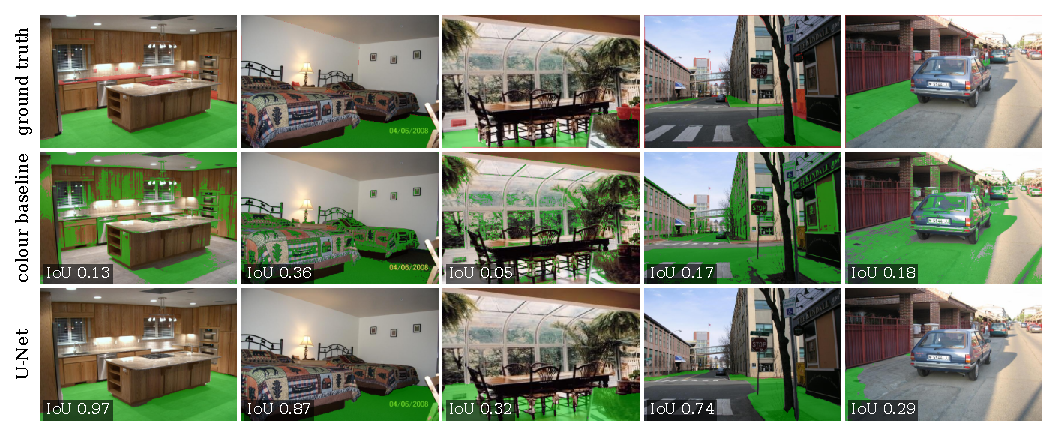
\includegraphics[width=0.86\linewidth]{qualitative.pdf}
  \caption{Validation examples with per-image IoU: U-Net 90th/50th/10th-percentile images, then two street scenes.}
  \label{fig:qualitative}
\end{figure}

\textbf{Challenges.} Sidewalk and road look alike but are labelled differently, and some labels
(crosswalk = road) disagree with where a pedestrian can walk. A more defined rule needs to be made to better
constrain how the model decides whether a floor surface is walkable or not.

\textbf{Feasibility.} The pipeline produces a functional segmentation, with training occurring in just 48 minutes.
What remains is feasible so long as the self labeled dataset is of reasonable size. 
From there I can begin initial attempts of video passthrough of the model, mobile deployment, and 
Google Maps navigation integration.

% =====================================================================
\clearpage   % references on a new page, after every figure
\bibliographystyle{unsrtnat}
\bibliography{references}

\end{document}
